\documentclass[11pt,a4]{article}
\usepackage{amssymb}
\usepackage{amsmath}
\usepackage[latin1]{inputenc}
\usepackage[top=3cm,bottom=2cm,left=2.0cm,right=2.0cm]{geometry}	
%\usepackage[portuguese]{babel}
\usepackage[english]{babel}
\usepackage{pstricks}
\usepackage{verbatim}
\usepackage{multicol}
\usepackage{graphicx}
\usepackage{graphics}
\renewcommand{\baselinestretch}{1.5}
\setlength\columnsep{15pt}

\begin{document}

\title{TTSP - Tagus Time Synchronization Protocol }
\author{Hugo Miguel Pinho Freire\\
\textit{Under supervision of Prof. Doutor Rui M. Rocha}\\ % supervisor
\textit{IST - Taguspark, Porto Salvo, Portugal}}
\maketitle
\begin{abstract}
The need for time synchronization in Wireless Sensor Networks (WSNs) is critical for accurate time-stamping of events, coordination of duty cycles and MAC layer protocols. Typical time synchronization protocols for WSNs tend to deliver a time precision that in many times is higher than required, thus, in such times, these protocols tend to waste vast amounts of valuable resources trying to achieve a time precision that is not required. We here, purpose Tagus Time Synchronization Protocol (TTSP), a time synchronization protocol with a cross-layered architecture, that adaptively delivers the required time precision. The proposed protocol was implemented in TinyOS and deployed in the Tagus-SensorNet, a WSN testbed in IST-TUL Taguspark campus main building.
\end{abstract}

\bigskip
\textbf{\Large Keywords:} Wireless Sensor Networks, Time Synchronization, TTSP
\bigskip
\begin{multicols}{2}
%
\section{Introduction}

% keywords: Wireless Sensor Networks
The development of Wireless Sensor Networks (WSNs)  has become one of the major enabling technologies for ubiquitous environments \cite{karl05}, that is, the capability of making use of seamless integrated technology in our surroundings in order to make them intelligent, thus, better serving our needs. By intelligent environment, we mean, an environment able to gather data, process local generated data, and actuate over that same environment. WSNs enables us to easily and cost-effective make this change in the environment.

% keywords: WSNs Applications
Typical WSNs applications are dedicated to closely observe real-world phenomena. One important operation on collecting data from a WSN is \textit{data aggregation}. The aggregation of individual sensor readings is possible only by exchanging messages that are timestamped by each sensor's local clock. This clearly mandates for a \textit{common notion of time} among the sensor nodes. However, not only WSN applications but also many of the networking protocols used in WSNs need this common notion of time. Prime examples are Medium Access Control (MAC) protocols based on Time Division Multiple Access (TDMA) or MAC protocols with coordinated wake up.

% keywords: Time Synchronization Requirements
We have seen by now that WSNs applications and network protocols have in fact requirements for a common notion of time. Protocols that provide such a common notion of time are clock synchronization protocols. In the past, researchers have developed successful  clock synchronization protocols for wired networks. These are unsuitable for a wireless sensor environment because the challenges posed by WSNs are different and manifold; to name a few, limited energy and bandwidth, limited hardware, latency, and unstable network conditions by mobility of sensors, dynamic topology, and multi-hopping. Regarding the available time synchronization protocols specifically for WSN, the choice of picking the most suitable can be quite peculiar. All of them, tend to fill the necessary requirements of a WSN time synchronization protocol, but fail, by seeking time precisions that are not required by their applications.

% keywords: Adaptive Time Synchronization, Motivation, Goals
Having realized the inadequacy of existing synchronization approaches, there was a need to develop Tagus Time Synchronization Protocol (TTSP), a simple, yet scalable and energy-efficient solution to the problem of timing synchronization in sensor networks that is flexible enough to meet the desired levels of time precision and algorithmic overhead. TTSP is purposed here as an adaptive approach to time synchronization which seeks to achieve a network wide synchronization in a scalable fashion way with application/MAC layer protocol specific precision while making an efficient use of the available network resources. This means that the synchronization protocol will prevent itself from wasting valuable network resources in order to deliver a precision that clearly exceeds the application/MAC layer protocol demand or its not even suitable. This approach shall free valuable resources and ultimately contribute to saving energy, therefore extending the network's useful life-time.

% keywords: Document Structure
The remainder of this extended abstract is organized into three main sections. The following section, section two, provides a detailed view of the proposed architecture. Section three provides an objective validation of TTSP's functionality, while, section four draws some final conclusions.

\begin{figure*}[!htb]
\begin{center}
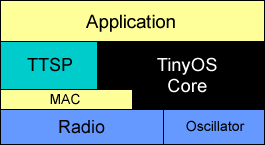
\includegraphics[scale=0.5]{./images/02-ttsp-hwsf_arch.png}
\end{center}
\caption{TTSP design goals.}
\label{designgoals}
\end{figure*}

\section{TTSP Design}

%-----------------------------------------------------------
% keywords: design goals
%-----------------------------------------------------------
For the design goals, we'll start by looking at Figure \ref{designgoals}, where we can easily see the different layers between the hardware and software components that occur in a sensor node and those that shall happen with TTSP. TTSP shall interface directly with the application and the MAC protocol for the desired time precision it needs to its correct operation. The application and the MAC protocol will be able to declare its time precision requirements to TTSP, and TTSP shall give feedback to the application if those requirements are successfully achieved. TTSP shall also interact with the available operating system running on the node, in this case, the TinyOS core, in order to access the time counters incremented by the oscillator and make use of the radio. These cross-layer interactions will allow TTSP to assure a global and unique notion of time synchronization to all components in the nodes system.

%-----------------------------------------------------------
% keywords: system architecture
%-----------------------------------------------------------
TTSP allows its cross-layers applications to declare their time precision requirements, by stating their tolerable time precision error. These requirements are to be managed by an adaptive synchronization layer, which encapsulates all the adaptive logic, that is, contains the adaptive algorithm, maintains the state of the current precision error, synchronization period, reference clock node and requirements declared by its clients. This adaptive synchronization layer operates over two other classic synchronization layers: pair-wise synchronization and network-wide synchronization. Each one of these two layers encapsulates their own synchronization logic, that is, implement the algorithms for pair-wise and network-wide synchronization, and both are controlled by the adaptive synchronization layer. These two layers export a set of commands and events that allow the upper layer to take full control of the time synchronization techniques.

%-----------------------------------------------------------
% keywords: pair-wise synchronization
%-----------------------------------------------------------
For pair-wise synchronization, TTSP uses a Sender-to-receiver message exchange scheme, mainly due to its low complexity and easy implementation. This pair-wise synchronization will be refreshed periodically. By using a MAC-layer time-stamping with an approach like Sender-to-receiver, the high delay uncertainty found in this type of approach when compared with a Receiver-to-receiver, clearly decreases. Making it a good choice instead of a Receiver-to-receiver with its inherent complexity.  By combining multiple estimates of the local time of a remote sensor node and using interpolation techniques it will be possible to compensate local clock skews.

%-----------------------------------------------------------
% keywords: network-wide synchronization
%-----------------------------------------------------------
For network-wide synchronization, the approach used for synchronization throughout the network is a master-slave scheme mainly also due to its low complexity and easy prediction of its behaviour while comparing to a peer-to-peer approach. The master will broadcast its local time to its neighbours, once these neighbours get synchronized with this master, they will then also start broadcasting to their neighbours.  In order to provide some redundancy to the master and easily adapt to network topology changes, a simple master election algorithm will ensure that a new root is elected once the previous one has cease to broadcast its local clock.

%-----------------------------------------------------------
% keywords: adaptive synchronization
%-----------------------------------------------------------
A periodic re-synchronization is needed, otherwise the timing of different nodes would drift apart as time passes. Thus, one needs to take into account that a less frequent re-synchronization requires a lower number of exchanged messages, thus, eventually lesser energy consumption by the sending and receiving nodes, but ultimately leads to a larger synchronization error, that is, time precision error. While a more frequent re-synchronization leads to a smaller time precision error but requires more energy. There is clearly a trade-off between energy expenditure and the achieved time precision error. The proposed adaptive synchronization layer shall find the minimum re-synchronization frequency (or equivalently maximum re-synchronization period) that can meet the desired  synchronization precision. Therefore the adaptive synchronization layer is necessary to dynamically determine the re-synchronization period to be used in each round of synchronization based on the needed time precision error.

%-----------------------------------------------------------
% keywords: time precision error
%-----------------------------------------------------------
The adaptive synchronization must have knowledge of the required time precision error. As previously said, this precision error is declared by the cross-layer clients. Once the adaptive layer knows this value, it now needs to know how to systematically measure the current achieved time precision error. This measure is done at both the sender and the receiver. Each one should monitor this parameter in order to actuate over it. One of the advantages of the promiscuous physical medium and the fact that exchanged messages are broadcasted on it, has the advantage that, in this case, the root node can listen to and measure the precision error of the synchronization messages of its synchronized nodes. In a multi-hop scenario these precision errors are obtained through relayed messages by the intermediary nodes. These intermediary nodes, which by then are already synchronized with the root node and aware of the time precision requirements are able to filter messages in case the calculated precision error is acceptable. Thus, in a multi-hop scenario the intermediary nodes have the responsibility of letting the root node know about unacceptable precision errors in the edges of the network. On the other side, the receiver has a lesser significant responsibility but still important of managing the synchronization points already collected and employ filtering techniques on them, in order to assure an acceptable time precision error. This management is needed since, while adjusting to a new synchronization period, the already collected number of samples might induce some small precision error when calculating the logical clock time.

%-----------------------------------------------------------
% keywords: synchronization period
%-----------------------------------------------------------
The root node has the responsibility of adjusting the synchronization period. The initial synchronization period is statically pre-configured on all nodes, and should reflect a period that is known to be safe to start with. The following synchronization periods to be used by the root node are adjusted by the adaptive algorithm, which reflect the current time precision error. This adaptive adjustment is made on the sole basis of the current time precision error. The adjustment is made using a Multiplicative Increase, Multiplicative Decrease (MIMD) strategy. The concept is straightforward, if the current time precision error is larger than  the requested time precision, it means that the synchronization period is too high, therefore the synchronization period should decrease by a certain factor. On the other hand, if the time precision error is smaller than the requested time precision error, that translates into a lower synchronization period, and thus, it could be increased by a certain factor. This adaptive algorithm can be best described by a state machine, in which is composed by three distinct states.

\begin{itemize}
\item Phase 1: the first and initial phase, is triggered on the root node after the first synchronization message from one of its receiving nodes is received, that is, once one neighbouring node gets synchronized and starts to broadcast its logical clock time. From that on, and on every synchronization message received in a synchronization round from its synchronized neighbours, the root adjusts the synchronization period to meet the required time precision error. The root node filters synchronization messages by its synchronization round identification, so that it only adjusts the synchronization period once in a synchronization round. Although, there are cases in which one node has an acceptable error, but another don't, in this case, the root needs to filter messages by synchronization rounds but also take into consideration the time precision error of the node, eventually giving priority to adjustments that keep the overall time precision error lower. For every two consecutive period increases, the algorithm records a safe period, which it will use as a fall-back when it receives a non-consecutive number of synchronization messages with an unacceptable precision error and needs to drastically decrease the synchronization period. The MIMD granularity used in this phase is typically higher than the other remaining phases, since there is no knowledge at that moment from the conditions of the network. The transition from this phase is done after a certain number of non-consecutive synchronization messages with a time precision higher than the accepted. When transitioning from this phase, the adaptive algorithm has the knowledge of the maximum synchronization period that it can sustain for the given network conditions. As said, this transition will be made after the maximum synchronization period is known, this will typically involve achieving a higher time precision error, which will result in a decrease in the time synchronization period to a known safe period, as previously explained. The next phase, will take this knowledge into consideration.

\item Phase 2: the second phase of the adaptive algorithm, is somehow similar with the first phase, it also can be described as a discovery phase, but now with the difference that we know the maximum synchronization period that can be achievable under an acceptable precision error, thus the MIMD granularity used in this phase is smaller than the used on the previous phase, since we're are interested in maximizing the synchronization period closer to the previous known maximum synchronization period but without the precision errors. Like in the previous phase, the algorithm quickly reacts to small variations of the achieved time precision error in order to keep it under the required precision. This phase is also considered a transition state, that is, the synchronization period can still fluctuate significantly between the two distinct thresholds that it knows, the safe synchronization period and the maximum synchronization period obtained from the previous phase. The transition from this phase is done after a certain number of consecutive increases and a decrease or a certain number of decreases and an increase.

\item Phase 3: the third and last phase of the adaptive algorithm can be considered a stabilization phase, since once in this phase the current synchronization period is considered safe and lower the maximum synchronization period where the unacceptable time precision errors were detected. In this phase, the MIMD granularity is very small since for most cases the precision error should be within the required thresholds and not be subject to high variations. This phase can be grossly characterized by a steady synchronization period. Nonetheless, if by any means, the time precision error keeps getting close to the threshold of the requested time precision error for a long period of time, that is, a certain number of synchronization round, a transition to phase two will be made, since it is considered that the current synchronization period is not suitable any more. The same procedure is made for when the time precision error is well below the requested time precision error and close to zero, but instead, a transition will be made to phase one, because of its higher MIMD granularity.
\end{itemize}

\section{TTSP Test and Evaluation}

\begin{figure*}[!b]
\begin{center}
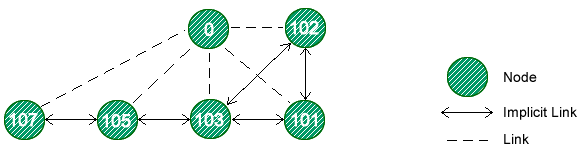
\includegraphics[scale=0.4]{./images/19-ttsp-test_topology.png}
\end{center}
\caption{Six nodes scenario with multi-hop synchronization.}
\label{scenario6}
\end{figure*}

%-----------------------------------------------------------
% keywords: Test-bed, Tests
%-----------------------------------------------------------
With the purpose of validating the proposed architecture, TTSP was deployed in a WSN test-bed and was subject to a series of scenario tests. These tests intend to evaluate the time synchronization in scenarios ranging from a single node to multiples nodes, from a single-hop network to a multi-hop network, from high precision requirements to much lower precision requirements. Since these tests were designed solely to show how TTSP's synchronization is effective and its features operate, in a qualitative manner, each test was run only once. Being this the case, the obtained results may only be used as a comparison between each test, since they lack the statistical relevance required to extrapolate reference performance values.\\
%-----------------------------------------------------------
% keywords: Tagus-SensorNet
%-----------------------------------------------------------
Regarding the test-bed, a WSN test-bed, Tagus-SensorNet \cite{pedrosa08}, allows the unique opportunity to test TTSP in a real deployment scenario, allowing it to experience the intrinsic constraints of a WSN. That is, in Tagus-SensorNet sensor nodes are faced with limited energy resources, communications that can easily be interfered and sensor nodes that can suddenly die or start functioning incorrectly.

%-----------------------------------------------------------
% keywords: Test Scenario
%-----------------------------------------------------------
The test scenario chosen for this purpose is described in Figure \ref{scenario6}. In this scenario, there are a total of five synchronizing nodes, of which, one node will be declared as the root node, four are to be synchronized with that root node at a given moment in time. One additional one node is used as a base-station for continuously collecting the selected metrics from the synchronized nodes and the root node. 

Although, most of the used nodes are in the radio coverage of each other, there was the need for a slightly different network topology that could best describe all the physical network topologies that are currently used by other applications in Tagus-SensorNet. For this reason, implicit links were statically configured in each node, which forced the desired logic topology as shown in the previous figure.

%-----------------------------------------------------------
% keywords: Test Results
%-----------------------------------------------------------
The processed test results will be presented and briefly discussed. The following indicators have been used across multiple tests:
\begin{itemize}
\item \textit{Precision Error}:  This value, as the name suggests, indicates the current time precision error achieved by a node when synchronized with the root node, measured in time units.
\item \textit{Synchronization Period}: This value indicates the current synchronization period being advertised by the root node to the synchronizing nodes, also measured in time units.
\end{itemize}

%-----------------------------------------------------------
% keywords: multi-hop/node synchronization with high precision requirements
%-----------------------------------------------------------
 For this test, it was requested from TTSP that the maximum precision error did not exceed the 10 ms. The obtained results in Figure \ref{10ms6nodes}.

\begin{figure*}[!t]
\begin{minipage}[b]{0.5\linewidth}
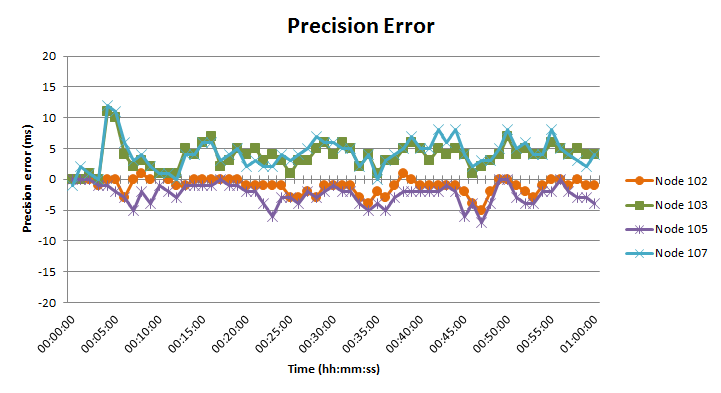
\includegraphics[scale=0.3]{./images/11-ttsp-10ms6nodes-error.png}
\end{minipage}
\hspace{0.5cm}
\begin{minipage}[b]{0.5\linewidth}
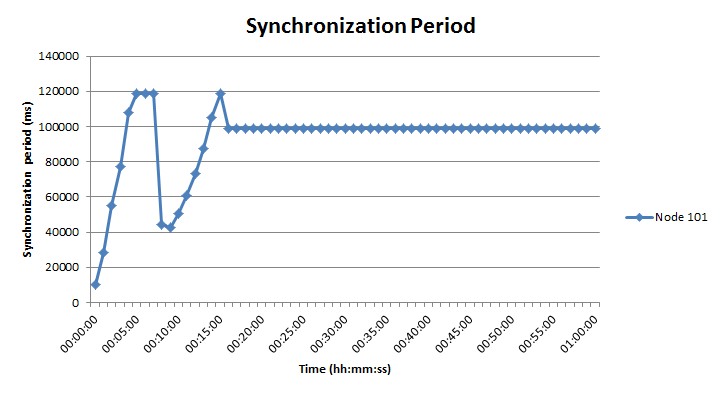
\includegraphics[scale=0.3]{./images/12-ttsp-10ms6nodes-period.png}
\end{minipage}
\caption{Time precision error with a precision request of 10 ms and using 6 nodes.}
\label{10ms6nodes}
\end{figure*}

The results clearly show that TTSP converged to an approximated synchronization period of 100 seconds, that assures that the requirement is fulfilled correctly. One must also note the time needed for this convergence, in this test, it was needed more than 15 minutes to TTSP finally converge to the fore mentioned synchronization period.

%-----------------------------------------------------------
% keywords: multi-hop/node synchronization with low precision requirements
%-----------------------------------------------------------
For the next experiment, the previous scenario was used, the only changed parameter as like the experiment with the single-node, was the maximum time precision error allowed in the network. Thus, the maximum tolerable precision error was increased to 50 ms. The obtained results can be seen in Figure \ref{50ms6nodes}.

\begin{figure*}[!t]
\begin{minipage}[b]{0.5\linewidth}
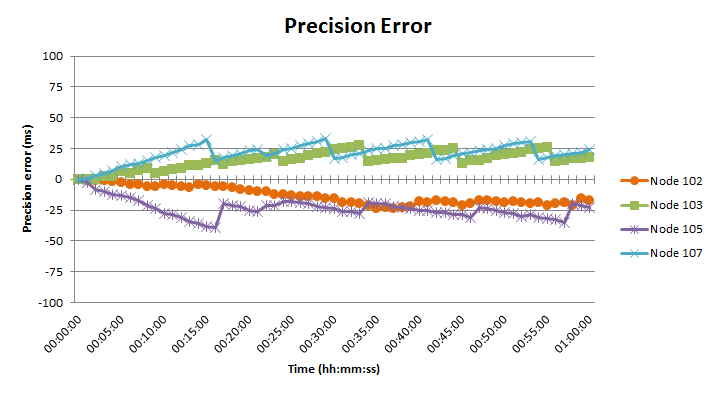
\includegraphics[scale=0.3]{./images/23-ttsp-50ms6nodes-error.png}
\end{minipage}
\hspace{0.5cm}
\begin{minipage}[b]{0.5\linewidth}
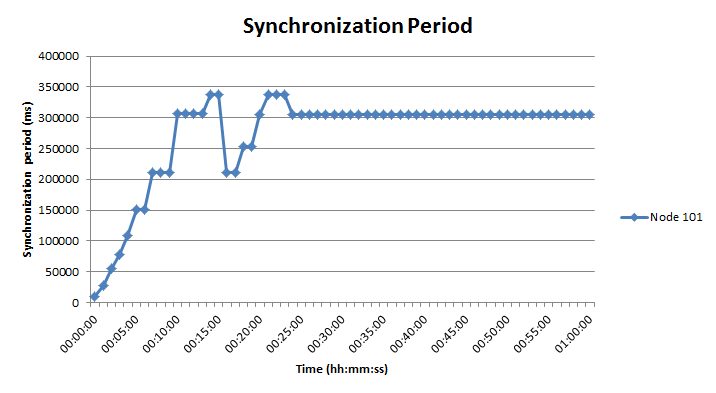
\includegraphics[scale=0.3]{./images/22-ttsp-50ms6nodes-period.png}
\end{minipage}
\caption{Time precision error with a precision request of 50 ms and using 6 nodes.}
\label{50ms6nodes}
\end{figure*}

From the results, it's possible to denote that the requirement is fulfilled and a synchronization period that best suits that requirement is found. Since the requirement was relaxed, it was expected that the synchronization period increased slightly, in this case for an approximated value of 300 seconds. With the relaxation of the requirement, it also resulted in a higher time interval finding the most suitable synchronization period, almost 25 minutes. This is mainly justified by the higher synchronization periods achieved, which result in longer times for feedback reception. 

%-----------------------------------------------------------
% keywords: fast synchronization mechanism
%-----------------------------------------------------------
The objective with the next experiment is to assess the fast synchronization mechanism that is triggered when for example a node joins the network for a first time after the synchronization period as already converged or the re-election mechanism has been triggered and the information of the new root is being propagated throughout the network. In Figure \ref{fastsync} it is possible to verify the obtained results with the use of this mechanism, it is important to point that the new node was turned on at exactly 40 minutes since the beginning of the test.

\begin{figure*}[!b]
\begin{minipage}[b]{0.5\linewidth}
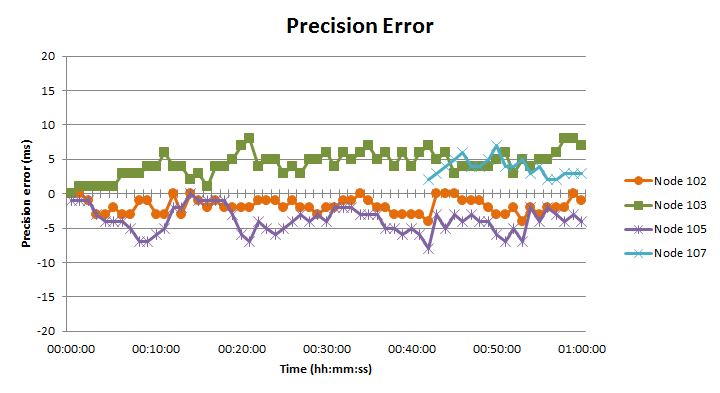
\includegraphics[scale=0.3]{./images/15-ttsp-10ms6nodes-fastsync-error.png}
\end{minipage}
\hspace{0.5cm}
\begin{minipage}[b]{0.5\linewidth}
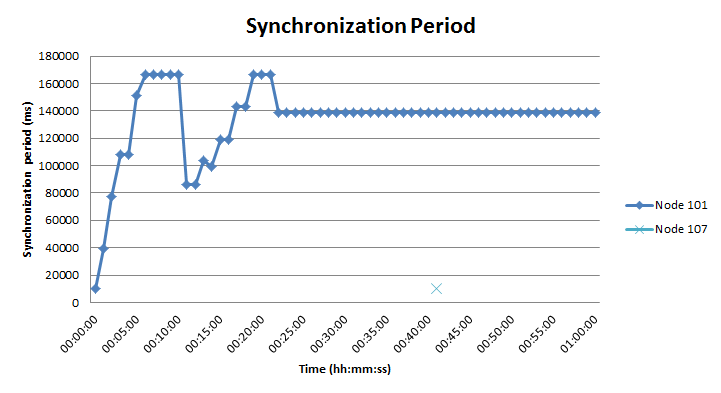
\includegraphics[scale=0.3]{./images/16-ttsp-10ms6nodes-fastsync-period.png}
\end{minipage}
\caption{Fast synchronization mechanism.}
\label{fastsync}
\end{figure*}

After the new node was turned on, and past the time duration of three times the initial synchronization period (in this case after 30 seconds) without hearing a synchronization broadcast. Once the new node elects himself, he starts to broadcast its local clock with a period of 10 seconds. The first broadcast is heard by its neighbouring nodes which triggers the fast synchronization mechanism, eventually leading the new node to be aware of the actual root node and become synchronized with it. 

%-----------------------------------------------------------
% keywords: re-election mechanism
%-----------------------------------------------------------
In the next experiment, the objective is to assess the re-election mechanism which must be executed once the current root node ceases to broadcast its local clock. The used scenario is the same as the one used with the multiple nodes and existence of multi-hop synchronization. The experiment is composed of a initial period where all synchronizing nodes will eventually synchronize with an elected root node, and consequently that root node will be remotely turned off, ceasing to broadcast its local clock. The remaining nodes, must continue to be synchronized among themselves, for that, the re-elections mechanism will be triggered and new root node elected. The results of this experiment can be seen in Figure \ref{reelection}.

\begin{figure*}[!t]
\begin{minipage}[b]{0.5\linewidth}
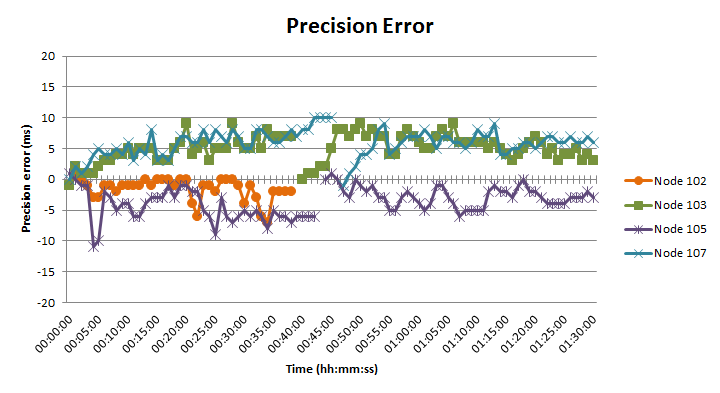
\includegraphics[scale=0.3]{./images/13-ttsp-10ms6nodes-reelection-error.png}
\end{minipage}
\hspace{0.5cm}
\begin{minipage}[b]{0.5\linewidth}
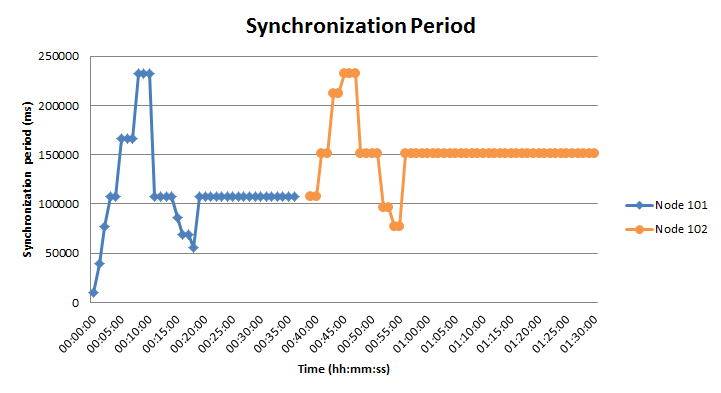
\includegraphics[scale=0.3]{./images/14-ttsp-10ms6nodes-reelection-period.png}
\end{minipage}
\caption{Re-election mechanism.}
\label{reelection}
\end{figure*}

The results are clear enough to tell that the new root node is elected, the remaining node with the lower identification. This process is triggered on each node after a root silence of three times the current synchronization period. In this case, 312000 ms after the first root node broadcasted its last local clock. After the re-election process is triggered,  the recent elected node continues with the same synchronization period than its predecessor, but becomes aware of the current low absolute precision error gathered from the synchronizing nodes and adaptively adjusts the synchronization period to a best suitable one.

\section{Conclusions}

We have described TTSP, an adaptive time synchronization protocol for WSNs. The results obtained with TTSP in Tagus-SensorNet make it a valid approach to synchronize clocks in WSNs. By using TTSP for time synchronization in a WSN, it's possible to adapt the time synchronization period to fulfil the time precision requirements while seeking to minimize the resource consumption in the process. TTSP also avoids statically pre-configured synchronization periods which might end not being suitable if for any reason the network topologies changes or nodes get removed or added to the network. TTSP cleverly finds the adequate synchronization period for the requested maximum time precision error allowed in the network, thus avoiding network administrator parametrization. One can also conclude that by using TTSP, it will be possible to maximize the network lifetime, since the most power demanding component of a node, the radio used for message transmission and reception is less used when a better suitable (obtained with TTSP) synchronization period is used. Finally, TTSP accomplishes the initial proposed goals, that is to achieve a network-wide synchronization in a scalable fashion way with requested specific time precision requirements while making an efficient use of the available network resources.

\begin{thebibliography}{100}
\bibitem{pedrosa08} Luis D. Pedrosa, Pedro Melo, Rui M. Rocha, Rui Neves. A flexible approach to WSN deployment. In Proceedings of The First International Workshop on Sensor Networks (SN´08), August, 2008.
\bibitem{karl05} H. Karl, A. Willig. Protocols and architectures for wireless sensor networks. Hoboken, NJ : Wiley, c2005.
%\bibitem{bulusu05} N. Bulusu, S. Jha. Wireless sensor networks: a systems perspective. Boston, MA : Artech House, 2005.
%\bibitem{palchaudhuri04} PalChaudhuri, S., Saha, A., and Johnson. Adaptive clock synchronization in sensor networks. In Proceedings The Third International Symposium on Information Processing in Sensor Networks (ISPN´04), 2004.
%\bibitem{qunli04} Qun Li, Daniela Rus. Global clock synchronization in sensor networks. In IEEE InfoCom, 2004.
%\bibitem{schenato07} L. Schenato and G. Gamba. A distributed consensus protocol for clock synchronization in wireless sensor network.  In 46th IEEE Conference on Decision and Control (CDC´07), 2007.
%\bibitem{ping03} S. Ping. Delay measurement time synchronization for wireless sensor networks. In Intel Research, IRB-TR-03-013, June 2003.
%\bibitem{solis06} R. Solis, V. Borkar, and P. R. Kumar. A New Distributed Time Synchronization Protocol for Multihop Wireless Networks. In Proceedings of 45th IEEE Conference on Decision and Control (CDC´06), 2006.
%\bibitem{maroti04} M. Maróti, B. Kusy, G. Simon, and Á. Lédeczi. The flooding time synchronization protocol. In Proceedings of the Second ACM Conference on Embedded Networked Sensor Systems (SenSys´04), 2004.
%\bibitem{greunen03} J. van Greunen, J. Rabaey. Lightweight time synchronization for sensor networks. in Proceedings of The Second ACM Int. Workshop on Wireless Sensor Networks and Applications (WSNA´03), September, 2003.
%\bibitem{elson02} Elson, J. E., Girod, L., and Estrin, D. Estrin. Fine-grained network time synchronization using reference broadcasts. In The Fifth Symposium on Operating Systems Design and Implementation (OSDI´02), December, 2002.
%\bibitem{ganeriwal05} S. Ganeriwal, R. Kumar, S. Adlakha, M. Srivastava. Timing-sync protocol for sensor networks. In Proceedings of ACM SenSys. 2003.
%\bibitem{kunsun06} K. Sun, P. Ning, C. Wang, A. Liu, Y. Zhou. TinySeRSync: secure and resilient time synchronization in wireless sensor networks. In Proceedings of the 13th ACM Conference on Computer and Communications Security (CCS´06), November, 2006.
%\bibitem{dai04} H. Dai and R. Han, TSync: a lightweight bidirectional time synchronization service for wireless sensor networks. ACM SIGMOBILE Mobile Computing and Communications Review 8 (2004), 2004.
\bibitem{levis05} P. Levis, S. Madden, J. Polastre, R. Szewczyk, K. Whitehouse, A. Woo, D. Gay, J. Hill, M. Welsh, E. Brewer, and D. Culler. TinyOS: An operating system for wireless sensor networks. In Ambient Intelligence. Springer-Verlag, 2005.
%\bibitem{levis03} P. Levis, N. Lee, M. Welsh, and D. Culler. TOSSIM: Accurate and Scalable Simulation of Entire TinyOS Applications. In Proceedings of the First ACM Conference on Embedded Networked Sensor Systems (SenSys´03), November 2003.
\end{thebibliography}
\end{multicols}
\end{document}
